\documentclass{article}

\usepackage[utf8]{inputenc}
\usepackage[T1]{fontenc}
\usepackage[portuguese]{babel}
\usepackage{amsmath, amsthm, amssymb}
\usepackage{graphicx}
\usepackage{bbm}

\author{Esdras R. Carmo - 170656}
\title{Integrais Duplas sobre Regiões Gerais}
\date{\today}

% Comando para integral dupla sobre região R
\newcommand{\doubleint}[1] {\iint\limits_R #1 dA}

% Definição para os exemplos
\theoremstyle{definition}
\newtheorem{example}{Exemplo}[section]

\begin{document}
    \maketitle

    \section{Regiões}
        \subsection{Tipo 1}
            Uma região $R$ do tipo 1 é dada por:

            \begin{align*}
                R &= \{ (x, y) \in \mathbbm{R}^2 \mid a \leq x \leq b, g_1(x) \leq y \leq g_2(x) \}\\
            \end{align*}

            Sendo $g_1$ e $g_2$ contínuas em $[a, b]$. Temos a integral:

            \begin{align*}
                \doubleint{f(x,y)} &= \int_a^b \int_{g_1(x)}^{g_2(x)} f(x,y) dy dx
            \end{align*}

        \subsection{Tipo 2}
            A região é dada por $R$ da seguinte forma:

            \begin{align*}
                R &= \{ (x, y) \in \mathbbm{R}^2 \mid c \leq y \leq d, h_1(y) \leq x \leq h_2(y) \}
            \end{align*}

            Sendo $h_1$ e $h_2$ contínuas em $[c, d]$. Temos a integral:
            
            \begin{align*}
                \doubleint{f(x,y)} &= \int_c^d \int_{h_1(y)}^{h_2(y)} f(x,y) dx dy
            \end{align*}

    \section{Propriedades}
        Vale todas as propriedades das integrais duplas sobre retângulos. No entando, se $D = D_1 \cup D_2$, com
        $D_1 \cap D_2 = \emptyset$, ou seja, interior não se interceptam, então:

        \begin{align*}
            \iint\limits_D f(x,y) dA &= \iint\limits_{D_1} f(x,y) dA + \iint\limits_{D_2} f(x,y) dA
        \end{align*}

    \section{Área da Região}
        Sendo $R$ uma região plana, então sua área é dada por:

        \begin{align*}
            A(R) &= \doubleint{1}
        \end{align*}

    \section{Exemplos}
        \begin{example}
            Calcula $\doubleint{(x + 2y)}$, em que $R$ é a região limitada pelas parábolas
            $y = 2x^2$ e $y = 1 + x^2$.

            \paragraph{}
            Note a figura~\ref{graph:parabolas}.

            \begin{figure}[h!]
                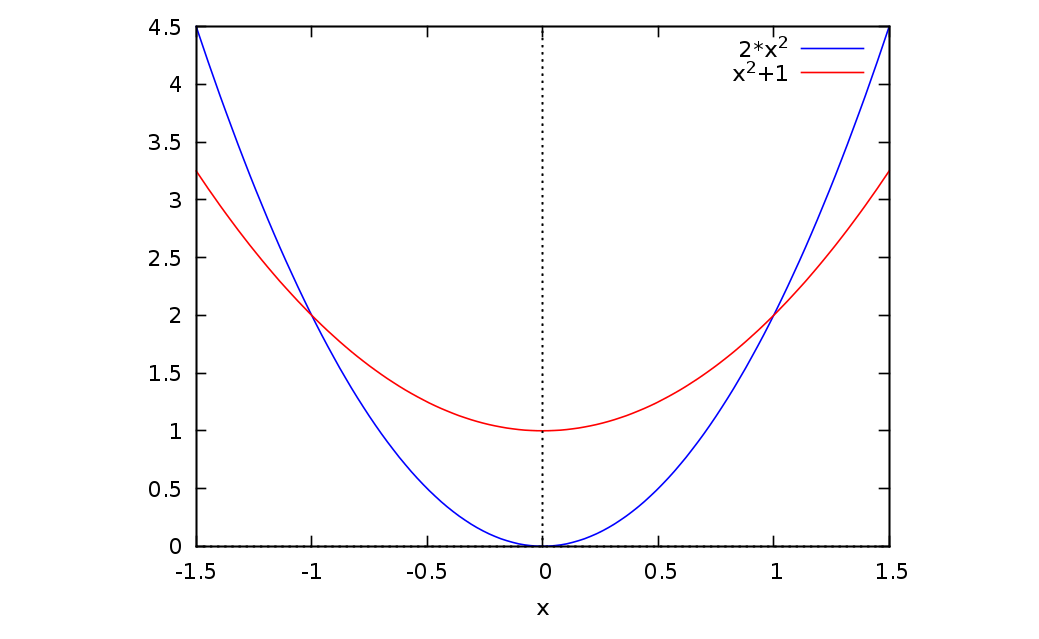
\includegraphics[width=\linewidth]{parabolas.png}
                \label{graph:parabolas}
                \caption{Gráfico das parábolas $y = 2x^2$ e $y = 1 + x^2$}
            \end{figure}

            Assim, temos $2x^2 \leq y \leq 1 + x^2$. Vamos encontrar:

            \begin{align*}
                2x^2 = 1 + x^2 \Rightarrow x = \pm 1
            \end{align*}

            Portanto $-1 \leq x \leq 1$. Temos:

            \begin{align*}
                \doubleint{(x + 2y)} &= \int_{-1}^1 \int_{2x^2}^{1 + x} (x + 2y) dy dx\\
                &= \int_{-1}^1 \left[ xy + y^2 \right]_{2x^2}^{1 + x^2} dx\\
                &= \int_{-1}^1 \left[ 1 + x + 2x^2 - x^3 - 3x^4 \right] dy\\
                \doubleint{(x + 2y)} &= \left[ x + \frac{x^2}{2} + \frac{2x^3}{3} - \frac{x^4}{4} - \frac{3x^5}{5} \right]_{-1}^1 = \frac{32}{15}
            \end{align*}
        \end{example}

        \begin{example}
            Determine o volume do sólido que está abaixo do paraboloide $z = x^2 + y^2$ e acima da região $R$ do plano $xy$ limitada pela reta
            $y = 2x$ e parábola $y = x^2$.

            \paragraph{}
            Note a figura~\ref{graph:reta-parabola}.
            
            \begin{figure}[h!]
                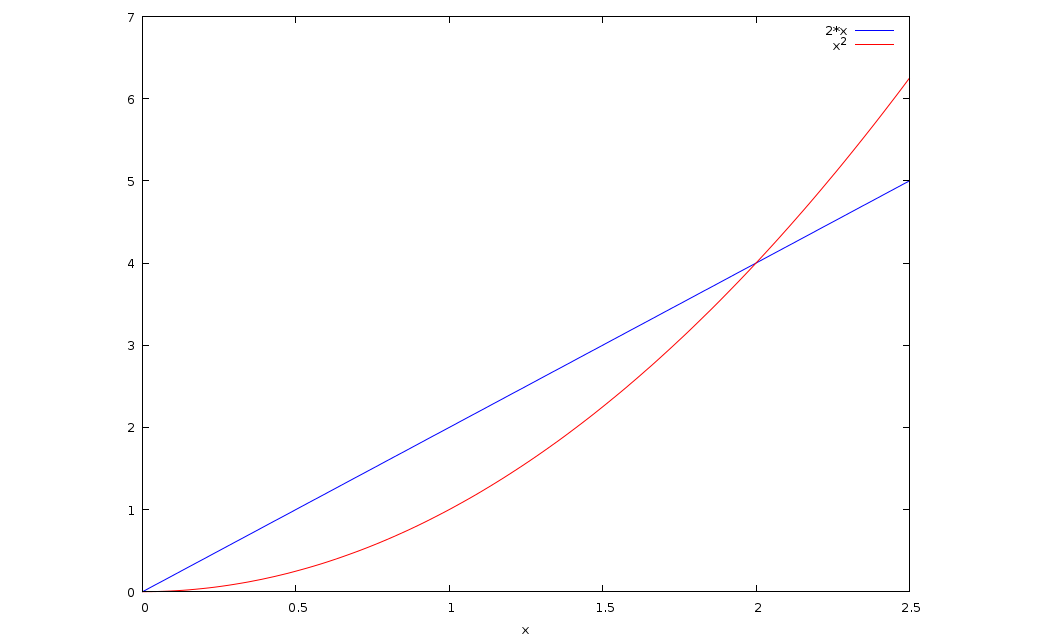
\includegraphics[width=\linewidth]{reta-parabola.png}
                \label{graph:reta-parabola}
                \caption{Gráfico da reta $y = 2x$ e parábola $y = x^2$}
            \end{figure}

            Assim, precisamos:

            \begin{align*}
                2x &= x^2 \Rightarrow x^2 - 2x = 0 \Rightarrow x = 0, x = 2\\
                0 &\leq x \leq 2\\
                x^2 &\leq y \leq 2x
            \end{align*}

            Assim, temos:

            \begin{align*}
                \doubleint{(x^2 + y^2)} &= \int_0^2 \int_{x^2}^{2x} (x^2 + y^2) dy dx\\
                &= \int_0^2 \left[ x^y + \frac{y^3}{3} \right]_{x^2}^{2x}\\
                &= \int_0^2 \left[ \frac{14}{3}x^3 - x^4 - \frac{x^6}{3} \right] dx\\
                &= \left[ \frac{7x^4}{6} - \frac{x^5}{5} - \frac{x^7}{21} \right]_0^2\\
                \doubleint{(x^2 + y^2)} &= \frac{216}{35}
            \end{align*}
        \end{example}

        \begin{example}
            Calcule a integral iterada:
            
            \begin{align*}
                \int_0^1 \int_x^1 \sin{y^2} dy dx
            \end{align*}

            Verifique a mudança de região para o tipo 2:

            \begin{align*}
                \int_0^1 \int_x^1 \sin{y^2} dy dx &= \int_0^1 \int_0^y \sin{y^2} dx dy\\
                &= \int_0^1 \left[ x\sin{y^2} \right]_0^y dy\\
                &= \int_0^1 y\sin{y^2} dy
            \end{align*}

            Tome $u = y^2$, $du = 2ydy$, $u(0) = 0$ e $y(1) = 1$, então:

            \begin{align*}
                \int_0^1 \int_x^1 \sin{y^2} dy dx &= \int_0^1 \frac{\sin{u}}{2} du\\
                &= \frac{1}{2} \left[ -\cos{u} \right]_0^1\\
                \int_0^1 \int_x^1 \sin{y^2} dy dx &= \frac{1}{2} \left( 1 - \cos{1} \right)\\
            \end{align*}
        \end{example}
\end{document}
